
\documentclass[a4paper,12pt]{article}

\usepackage[a4paper, total={6in, 8in}, left=30mm]{geometry}
\usepackage{pdfpages}

\usepackage{cmap}
\usepackage{caption}
\usepackage[T2A]{fontenc}
\usepackage[utf8]{inputenc}
\usepackage[english,russian]{babel}
\usepackage{fancyhdr}
\usepackage{minted}
\usepackage{hyperref}
\usepackage{amsmath}
\usepackage{graphicx}
\usepackage[document]{ragged2e}

\providecommand{\tightlist}{%
  \setlength{\itemsep}{0pt}\setlength{\parskip}{0pt}}

\hypersetup{
  pdfborderstyle={/S/U/W 1}
}

\graphicspath{{./images/}}

\pagestyle{fancy}
\fancyhf{}
\lhead{Антон Завьялов, ПИ-72}
\rhead{\textbf{Лабораторная №2}}
\cfoot{\thepage}

\makeatletter
\def\@seccntformat#1{%
  \expandafter\ifx\csname c@#1\endcsname\c@section\else
  \csname the#1\endcsname\quad
  \fi}
\makeatother

\begin{document}
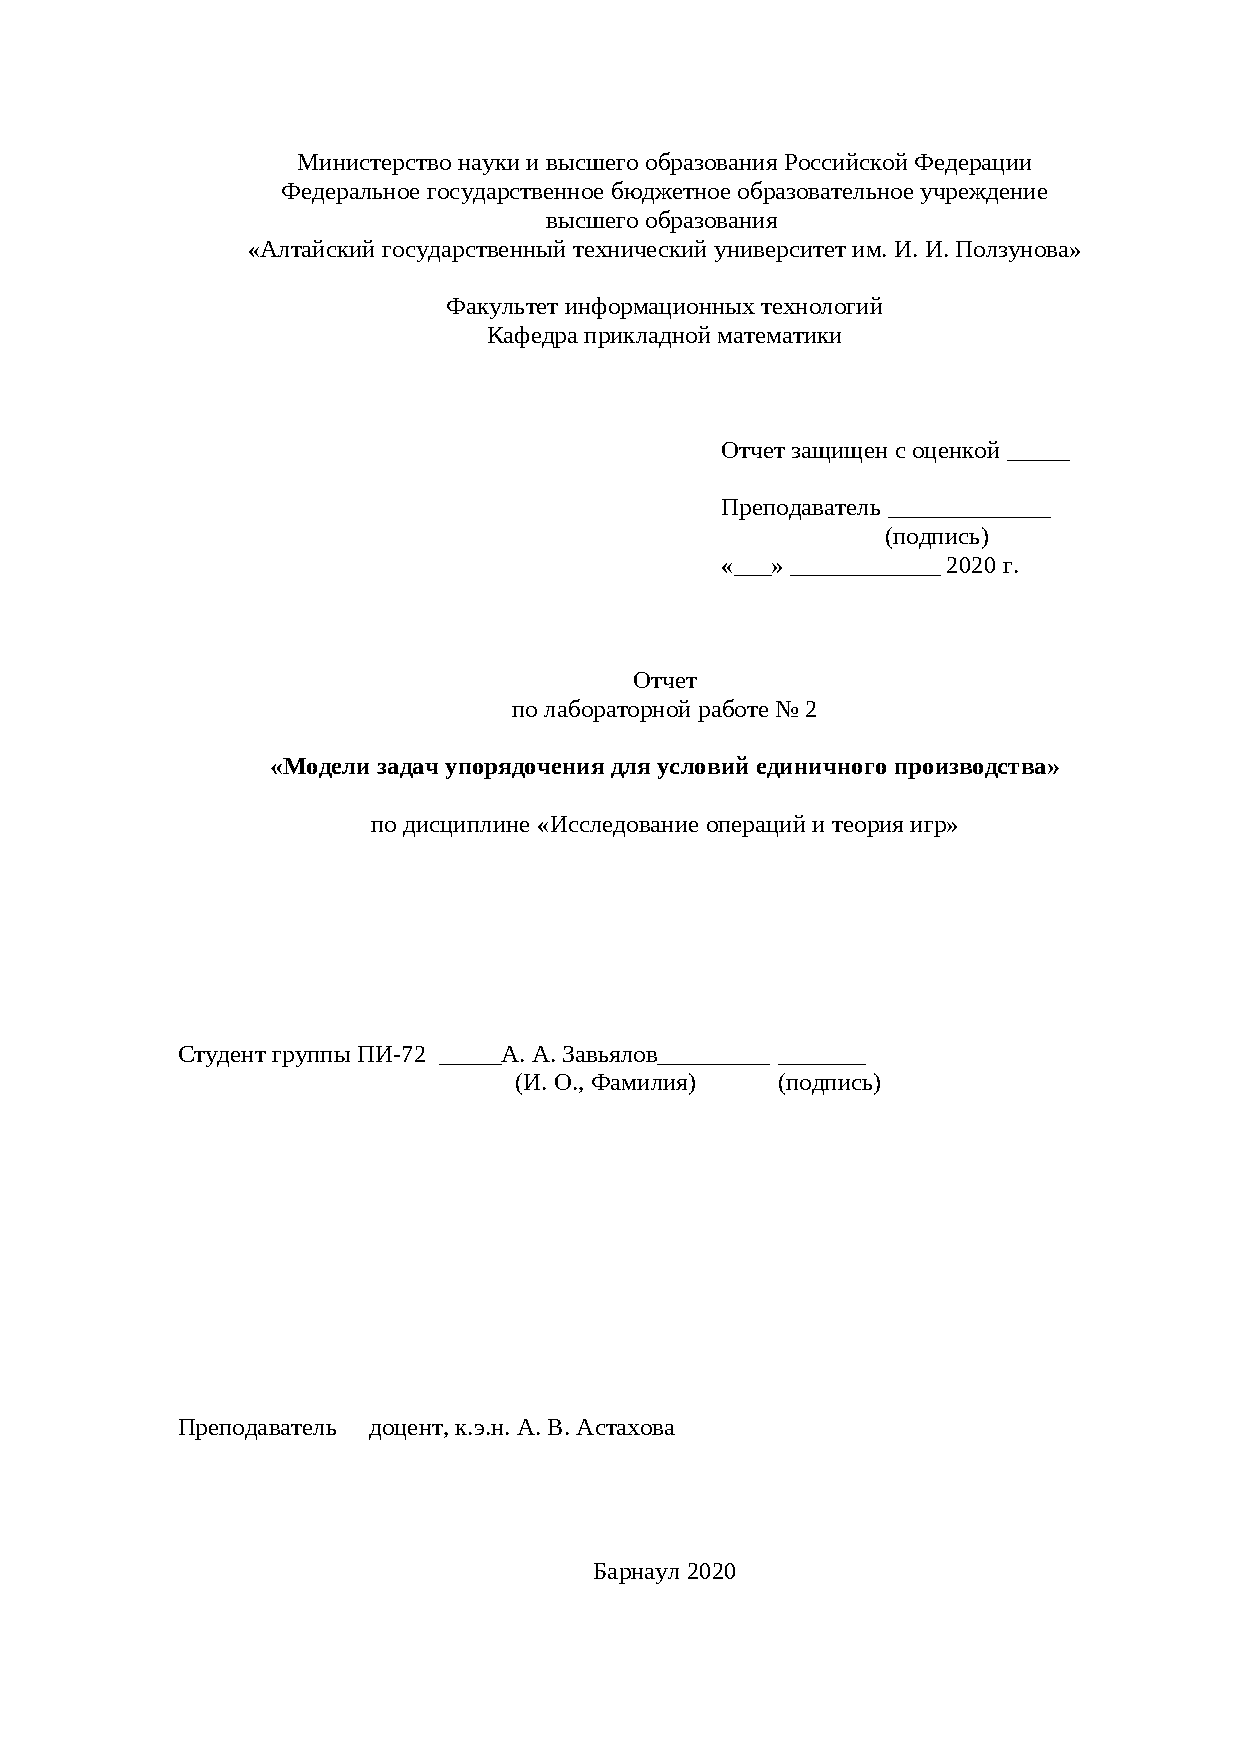
\includepdf[pages={1}]{title.pdf}

\section{\normalsize{Задание на лабораторную работу}}
\begin{flushleft}
\textbf{Задание 1. Построение графика Ганта для учебного примера Фишера
-Томпсона}
\justify
\begin{enumerate}
\item
  Ознакомиться с теоретическими основами решения задач теории расписаний
  для условий единичного производства, используя методические указания
  по теме. См. файл Module\_1\_Modeli\_zadach\_uporyadocheniya (в
  системе Илиас), пункт «Задачи упорядочения n$\times$m».
\item
  С помощью компьютерной программы Models или вручную на листе клетчатой
  бумаги, используя эвристический алгоритм запуска деталей в обработку,
  построить вариант графика Ганта загрузки 6 станков ($A$, $B$, $C$, $D$, $E$, $F$),
  являющийся технологически допустимым и отвечающим заданному
  ограничению по времени обработки всех 6 деталей \textbf{Т $\le$ 68} (ед.
  времени). Исходные данные для решения задачи заданы в двух таблицах $F$
  и $T$ на рис. 1. Номера строк обеих таблиц i -- соответствуют индексам
  (номерам) деталей; номера столбцов j -- соответствуют номерам
  технологических операций по маршруту. Значения элементов матриц F и Т
  соответственно: f\textsubscript{ij} -- шифр станка, на котором
  выполняется операция j делали i;\\
  t\textsubscript{ij}-- норма времени этой операции на данном станке. 

  Очевидно, что технологический маршрут по операциям детали i отображен в
  строке i матрицы F. Например, деталь № 2 при ее производстве проходит
  последовательно через обработку на станках В, C, E, F, А, D. Иная
  последовательность обработки, естественно, не допустима.

  При этом если, например, f\textsubscript{23 }= Е, то операция № 3 для
  детали № 2 выполняется на станке Е. Норма времени для нее
  t\textsubscript{23}= 10 (ед. времени) записана в матрице Т (нормы
  времени по операциям).

\item
  Определить следующие параметры построенного графика загрузки станков:

\begin{itemize}
\item
  длительность производственного цикла обработки всех деталей на всех
  станках;
\item
  время простоя каждого станка;
\item
  время «пролеживания» деталей в ожидании обработки на каждом станке. 
\begin{flushleft}\end{flushleft}
\begin{figure}
    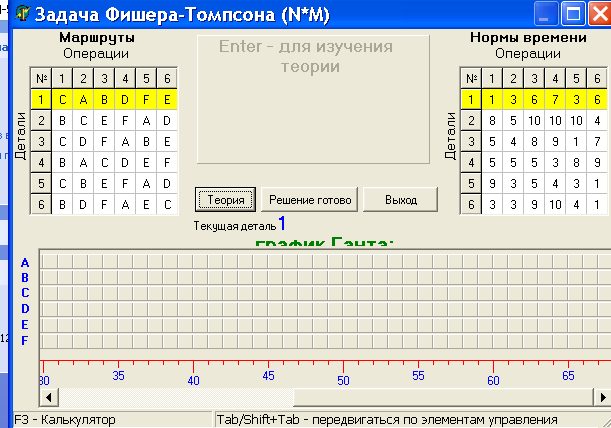
\includegraphics[width=8.832cm,height=6.156cm]{pic_1.png}
    \centering
    \caption{\small{Экранная форма при работе в пункте меню «Задача
    Фишера-Томпсона»}}
\end{figure}
\end{itemize}
\end{enumerate}
\raggedright
\textbf{Задание 2. Разработка алгоритма и программы имитационного
моделирования загрузки оборудования }
\justify
\begin{enumerate}
\item
  В соответствие с теоретическими основами решения задач теории
  расписаний для условий единичного производства (см. в Илиас параграф
  «Задачи упорядочения n$\times$m» в файле:
  Module\_1\_Modeli\_zadach\_uporyadocheniya), разработать алгоритм
  моделирования загрузки оборудования, взяв за основу принцип
  моделирования «по особым состояниям». 

  В алгоритме учесть процедуру упорядочения деталей в очереди с учетом
  выбора одного из двух заданных привила предпочтения запуска деталей в
  обработку -- в момент, когда у станка возникает очередь деталей.

  Вариант правил предпочтения, используемых при возникновении очереди
  деталей перед станком, задается преподавателем (см. файл «Правила
  предпочтения»). \textbf{Варианты: 3 - по длительности очередной операции (min), 12 - длительность части производственного цикла, операции по которому осталось выполнить (max).}

\item
  Составить и отладить программу на алгоритмическом языке (по выбору
  студента), одна из процедур которой выбирает деталь из очереди у
  станка (\emph{если} очередь образовалась) по заданному правилу
  предпочтения. На вход программы подается информация о размерности двух
  матриц F и Т, описанных выше; содержание матриц (возможны маршруты
  различной длины); «номер» правила предпочтения (для вызова
  соответствующей процедуры упорядочения). Длины технологических
  маршрутов деталей могут быть разными. В результате моделирования
  необходимо рассчитать три параметра (выбранные в качестве показателей
  эффективности) построенного графика загрузки станков:

  \begin{itemize}
  \item
    длительность производственного цикла Т обработки всех деталей на всех
    станках;
  \item
    время простоя каждого станка;
  \item
    время «пролеживания» деталей в ожидании обработки на каждом станке. 
  \end{itemize}

  Требование к интерфейсу программы: результатом работы программы должен
  быть график Ганта, выведенный на экран монитора компьютера (в форме
  линейной диаграммы), три параметры, его характеризующие; линейные
  диаграмма, моделирующие очереди деталей перед станками, возникающие в
  процессе моделирования (также выведенные на экран).

\item
  Запустив программу два раза (на одних и тех же исходных данных) с
  двумя различными правилами предпочтения, и получив два варианта
  загрузки станков, проанализировать полученные показатели эффективности
  модели. Сделать вывод, каким образом и почему (в Вашем конкретном
  случае) правило предпочтения влияет на показатели эффективности
  графика загрузки оборудования. 
\end{enumerate}
\end{flushleft}

\pagebreak

\section{\normalsize{Выполнение работы}}
\begin{flushleft}
\textbf{Задание 1. Построение графика Ганта для учебного примера Фишера
-Томпсона}
  \justify
  \begin{enumerate}
    \item Построен вариант графика Ганта загрузки 6 станков ($A, B, C, D, E, F$), являющийся технологически допустимым и отвечающим заданному ограничению по времени обработки всех 6 деталей \textbf{T $\le$ 68} (ед. времени):
    \begin{figure}[H]
      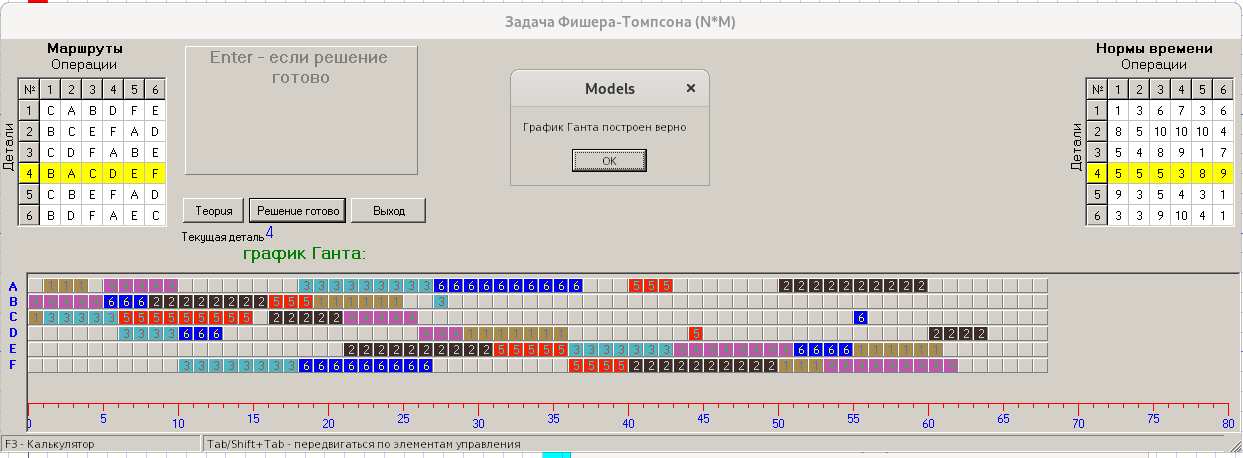
\includegraphics[width=15.25cm,height=6.5cm]{heuristics.png}
      \centering
      \caption{\small{График Ганта загрузки станков $A, B, C, D, E, F$}}
  \end{figure}
    \item Получены параметры графика загрузки станков:
    \begin{itemize}
      \item Длительность производственного цикла обработки всех деталей на всех станках: 64 (ед. времени);
      \item Время простоя каждого станка (ед. вр.):\newline A = 24, B = 38, C = 38, D = 42, E = 24, F = 43;
      \item Время «пролеживания» деталей в ожидании обработки на каждом станке (ед. вр.):\newline дет. 1 = 35, дет. 2 = 17, дет. 3 = 8, дет. 4 = 27, дет. 5 = 20, дет. 6 = 26.
    \end{itemize}
  \end{enumerate}
\end{flushleft}
\newpage
\begin{flushleft}
\textbf{Задание 2. Разработка алгоритма и программы имитационного
  моделирования загрузки оборудования }
  \justify
  \begin{enumerate}
    \item Разработан алгоритм моделирования загрузки оборудования на основе принципа "по особым состояниям":
    \begin{figure}[H]
      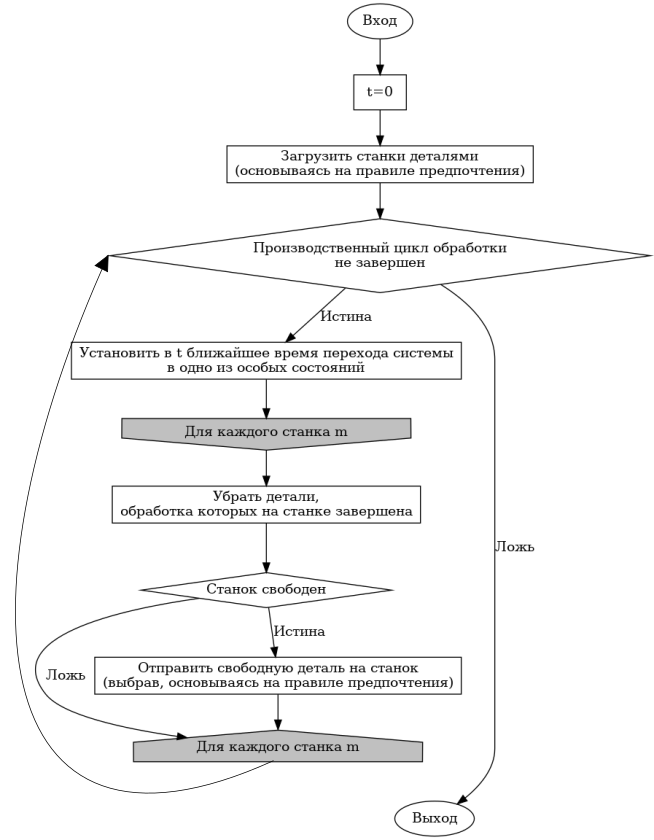
\includegraphics[width=15.25cm,height=15.5cm]{algorithm.png}
      \centering
      \caption{\small{Блок-схема алгоритма}}
  \end{figure}
  Упорядочение по правилу предпочтения легко спланировать, используя матрицы $F$, $T$. Введем дополнительные структуры данных:
  \begin{itemize}
    \item Матрица учёта прохождения технологических маршрутов $U$ с той же размерностью, что и у $F$, $T$. Изначально матрица заполнена единицами.
    \item Вектор занятости $B$ размера $m$, где $m$ - количество деталей в системе. Изначально заполнен нулями. Когда деталь $i$ поступает на станок, $i$-й элемент $B$ становится равным единице. При завершении обработки $i$-й детали, $i$-й элемент $B$ становится равен 0.
  \end{itemize}
  Тогда процедуру упорядочения для станка $k$ можно описать следующими шагами:
  \begin{enumerate}
    \item В каждой строке $i$ матрицы $U$ находится первое ненулевое значение и фиксируется пара индексов $ij$ этого элемента. Если таких элементов нет, очевидно, что производственный цикл завершён.
    \item Из всех полученных на прошлом этапе пар индексов $ij$ отсеиваются те, для которых в векторе занятости $B$ элемент по индексу $i$ равен единице (i-я деталь уже обрабатывается на одном из станков). Если в результате набор пар индексов стал пустым множеством, в текущий момент времени для станка $k$ выбрать деталь для обработки не можем (все детали заняты обработкой на других станках).
    \item В матрице маршрутов $F$ берутся все элементы по индексам $ij$, полученным на прошлом этапе, из них выбираются те пары $ij$, для которых элемент в матрице соответствует со станком $k$. Если таких элементов нет, значит, на текущий момент времени, детали либо не дошли до этапа обработки на $k$, либо уже прошли этот этап.
    \item Из результирующего множества индексов выбирается один по одному из правил предпочтения. В контексте работы: \begin{itemize}
      \item \textbf{По длительности очередной операции (мин.)}. Т.к. индексы $ij$ указывают на возможные очередные операции, достаточно выбрать такую операцию, для которой элемент в $T$ (матрица норм времени) по $ij$ (из ранее полученного множества индексов) будет минимальным.
      \item \textbf{Длительность части технологического цикла, операции по которому осталось выполнить (макс.)}. Строки матриц $F$, $T$ задают технологический маршрут обработки детали на станках и нормы времени обработки соответственно. Используя матрицу $U$ можно определить, доступна ли та или иная операция в будущем. Для всех $ij$ из множества ранее полученных индексов будем суммировать элементы строк $i$ начиная с индекса $j$ (первый из операций, которую осталось выполнить для детали $i$). Тогда достаточно выбрать такую операцию, однозначно определяемую индексами $ij$, для которой раннее полученная сумма будет \textbf{максимальной}.
    \end{itemize}
  \end{enumerate}
  \item Составлена программа на языке Python.\newline\linebreak
  \textbf{Исходный код программы}\newline\linebreak
  Исходный код ПО и код отчёта в системе вёртски \LaTeX $~$ доступен по ссылке: \url{https://github.com/andiogenes/iso/tree/master/lab_2}\newline\linebreak
  \textbf{main.py}
  \inputminted[breaklines]{python}{../main.py}
  \textbf{Формат входных данных}
  \inputminted[breaklines]{yaml}{../input.yaml}
  Здесь $F$ - матрица маршрутов, $T$ - матрица норм времени, rule - правило предпочтения (\textbf{FGFO} - по длительности очередной операции, \textbf{maxdistance} - Длительность части технологического цикла, операции по которому осталось выполнить (max)).\newpage
  \textbf{Тестовые примеры}\newline
  Медиафайлы из отчёта доступны для скачивания по ссылке:\url{https://github.com/andiogenes/iso/releases/download/1.2/lr2_full_scale.zip}
  \begin{enumerate}
    \item \item
    \begin{figure}[H]
      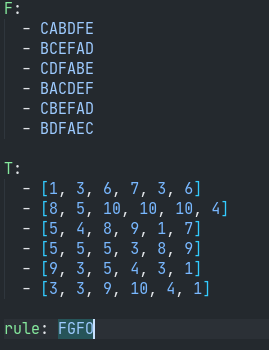
\includegraphics[width=5.25cm,height=6.5cm]{test_1_input.png}
      \centering
      \caption{\small{Модель из задания 1}}
    \end{figure}
    \begin{figure}[H]
      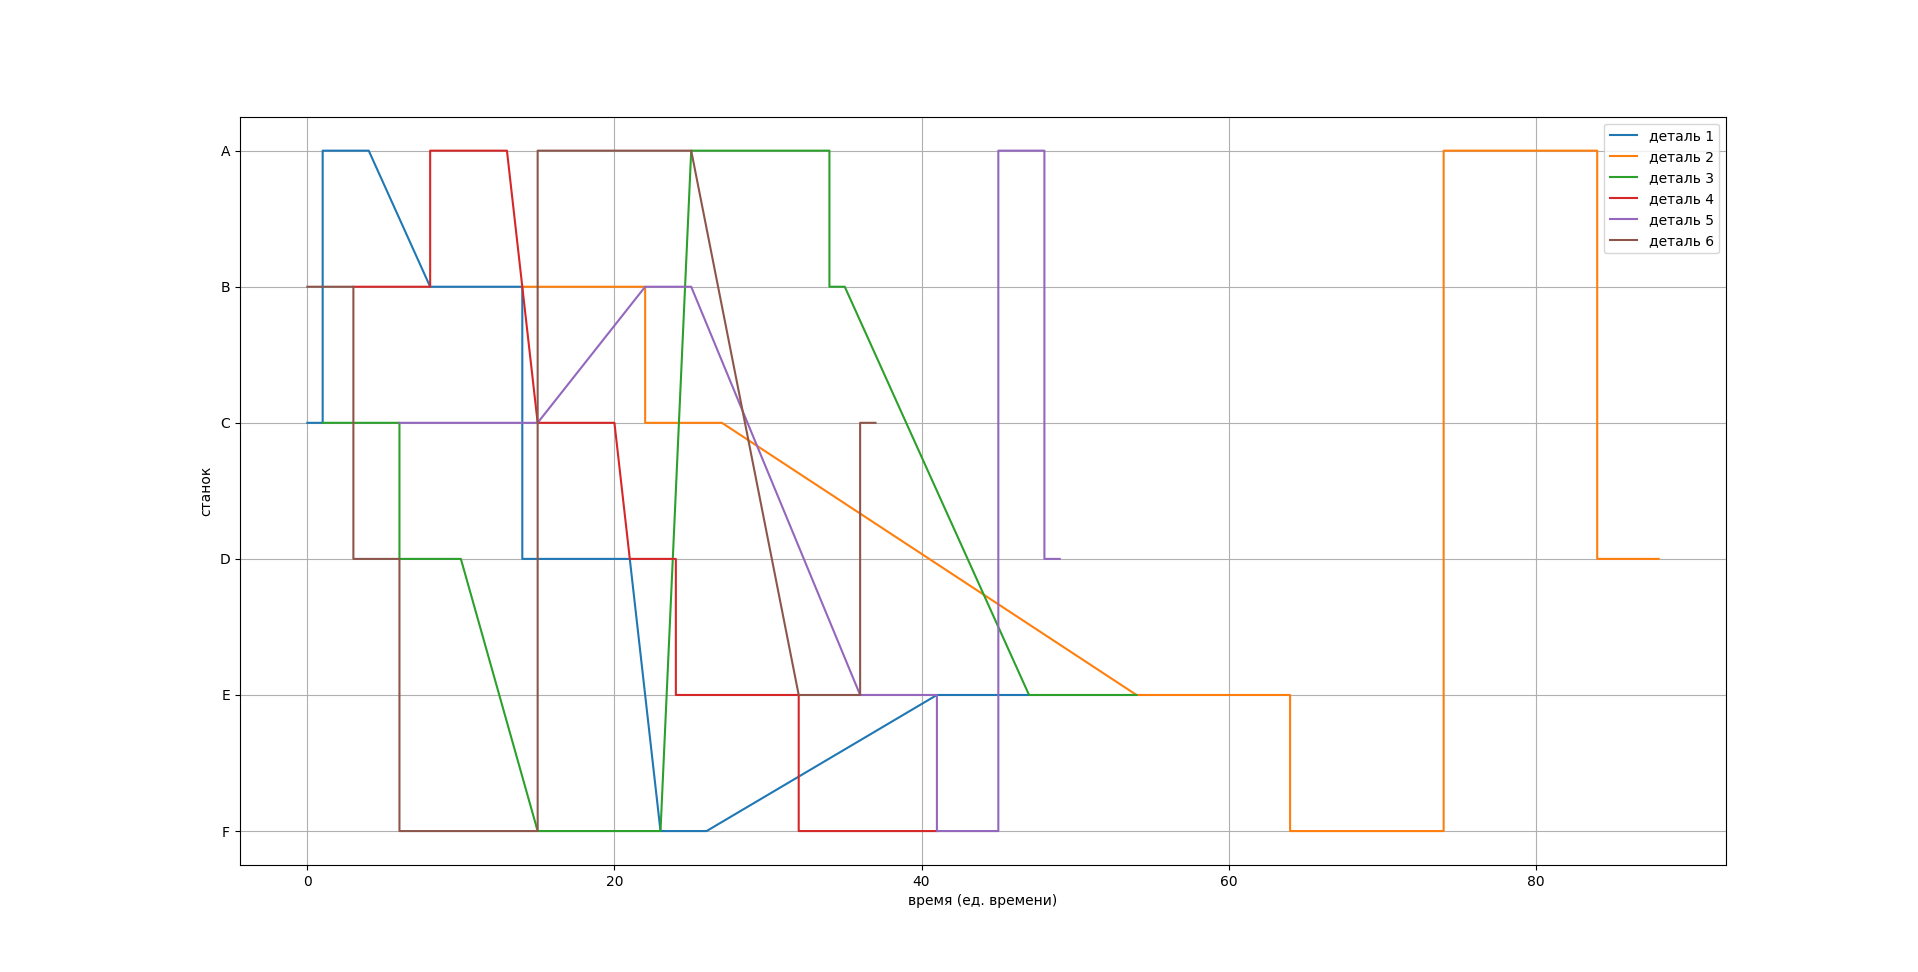
\includegraphics[width=18.25cm,height=8.5cm]{test_1.png}
      \centering
      \caption{\small{График Ганта в форме линейной диаграмы. На негоризонтальных участках графиков детали "пролеживают" до запуска на станок.}}
    \end{figure}
    \begin{figure}[H]
      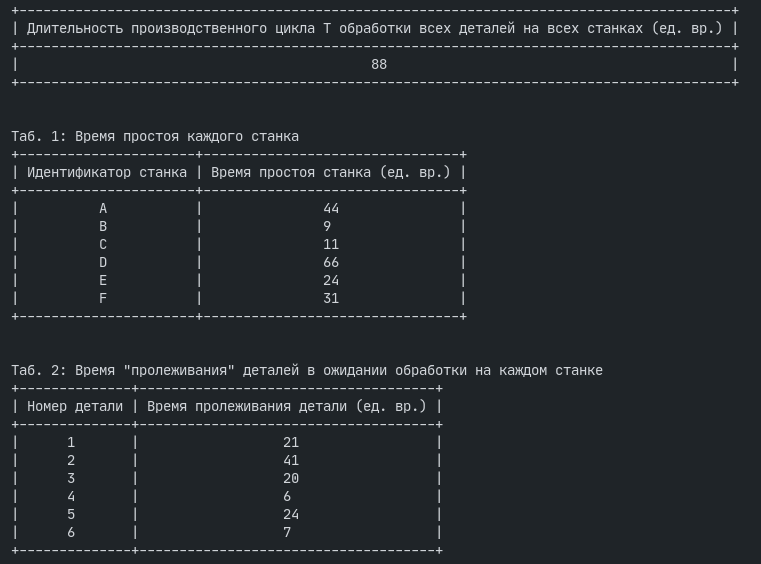
\includegraphics[width=12.25cm,height=8.5cm]{test_1_data.png}
      \centering
      \caption{\small{Параметры графика загрузки станков}}
    \end{figure}
    \item
    \begin{figure}[H]
      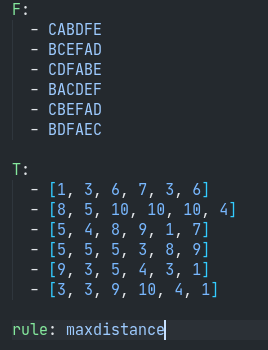
\includegraphics[width=5.25cm,height=6.5cm]{test_2_input.png}
      \centering
      \caption{\small{Та же модель с другим правилом предпочтения}}
    \end{figure}
    \begin{figure}[H]
      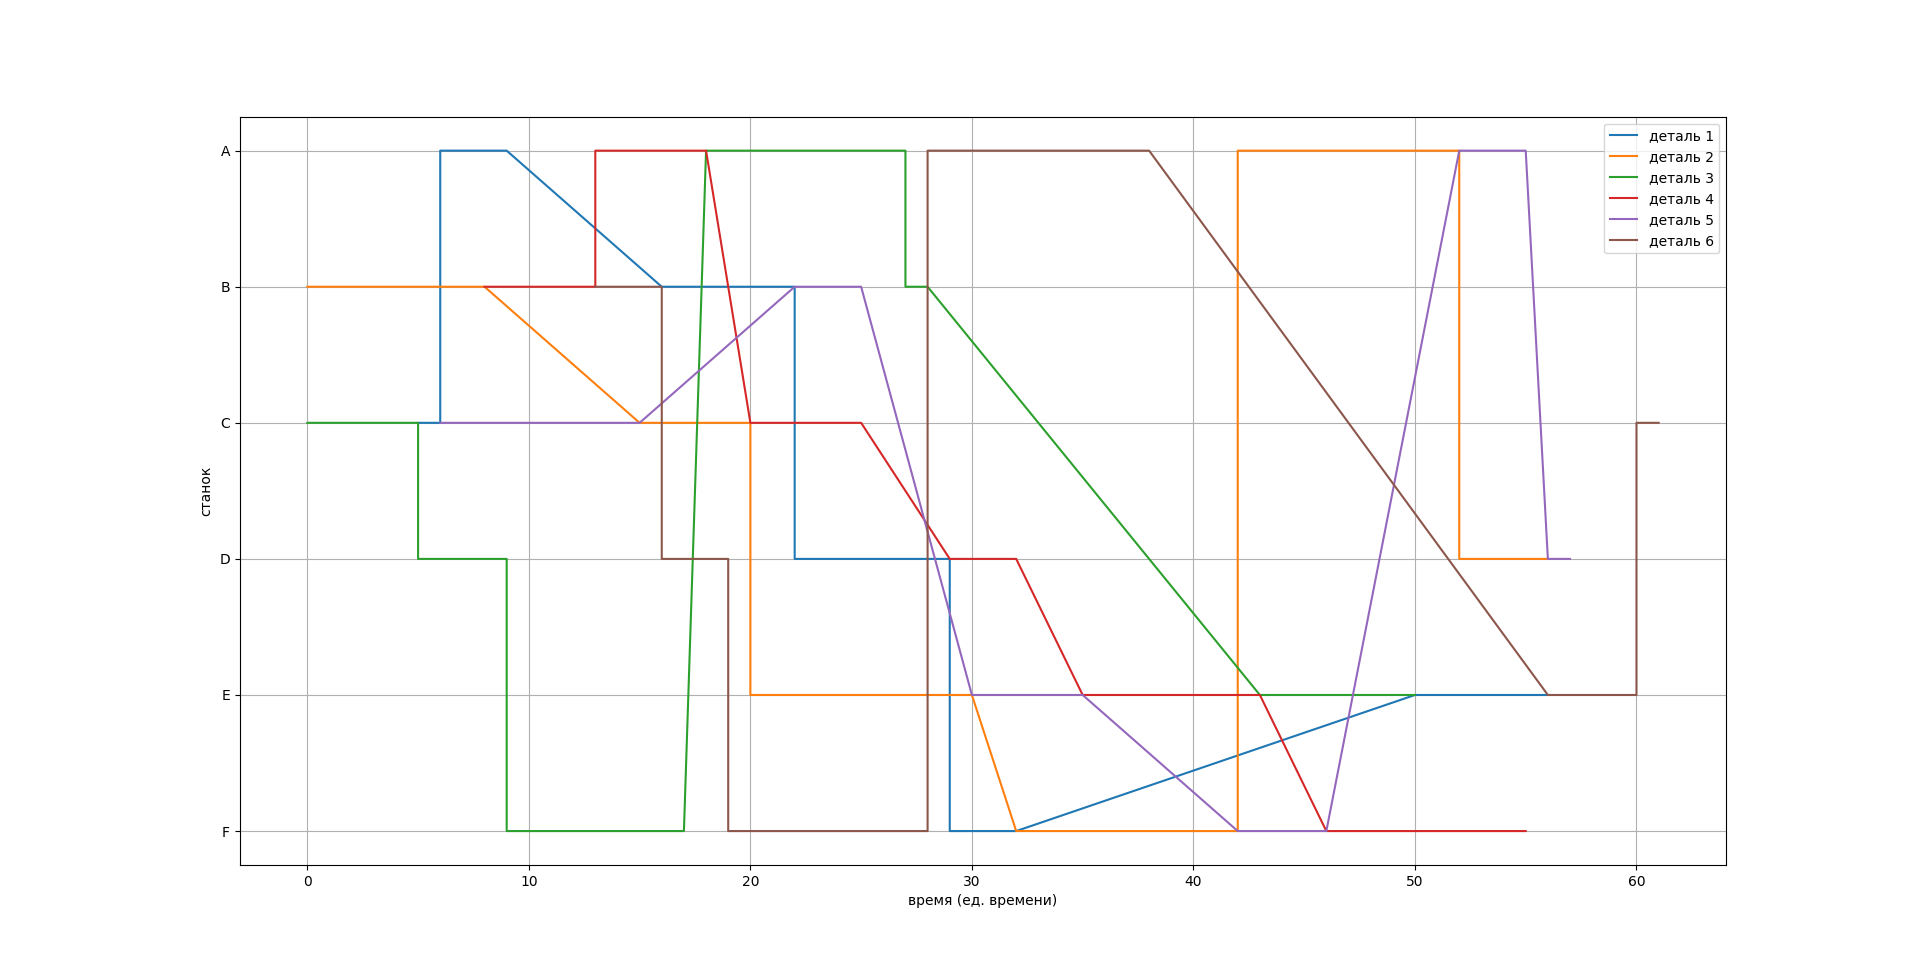
\includegraphics[width=18.25cm,height=8.5cm]{test_2.png}
      \centering
    \end{figure}
    \begin{figure}[H]
      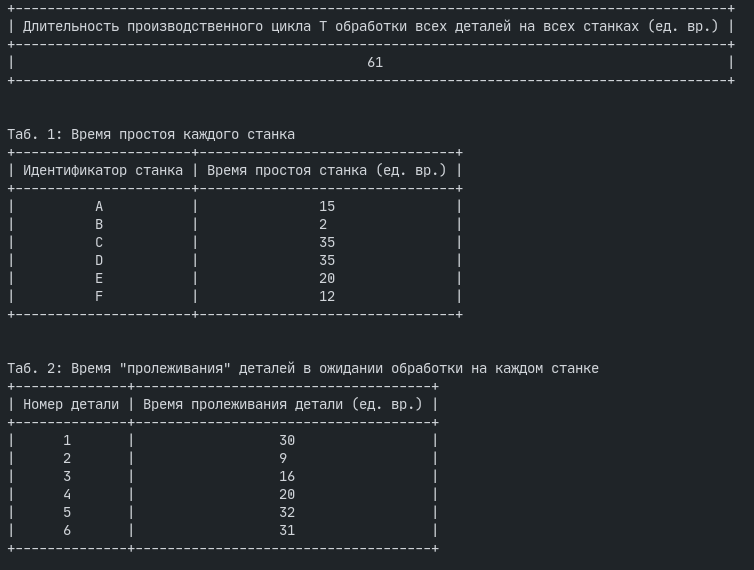
\includegraphics[width=12.25cm,height=8.5cm]{test_2_data.png}
      \centering
    \end{figure}
    \item
    \begin{figure}[H]
      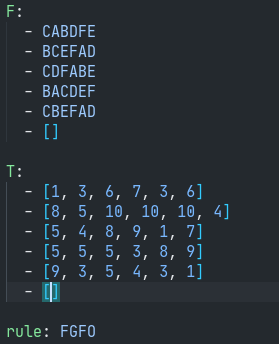
\includegraphics[width=5.25cm,height=6.5cm]{test_3_input.png}
      \centering
      \caption{\small{Модель с пустым технологическим маршрутом для детали 6}}
    \end{figure}
    \begin{figure}[H]
      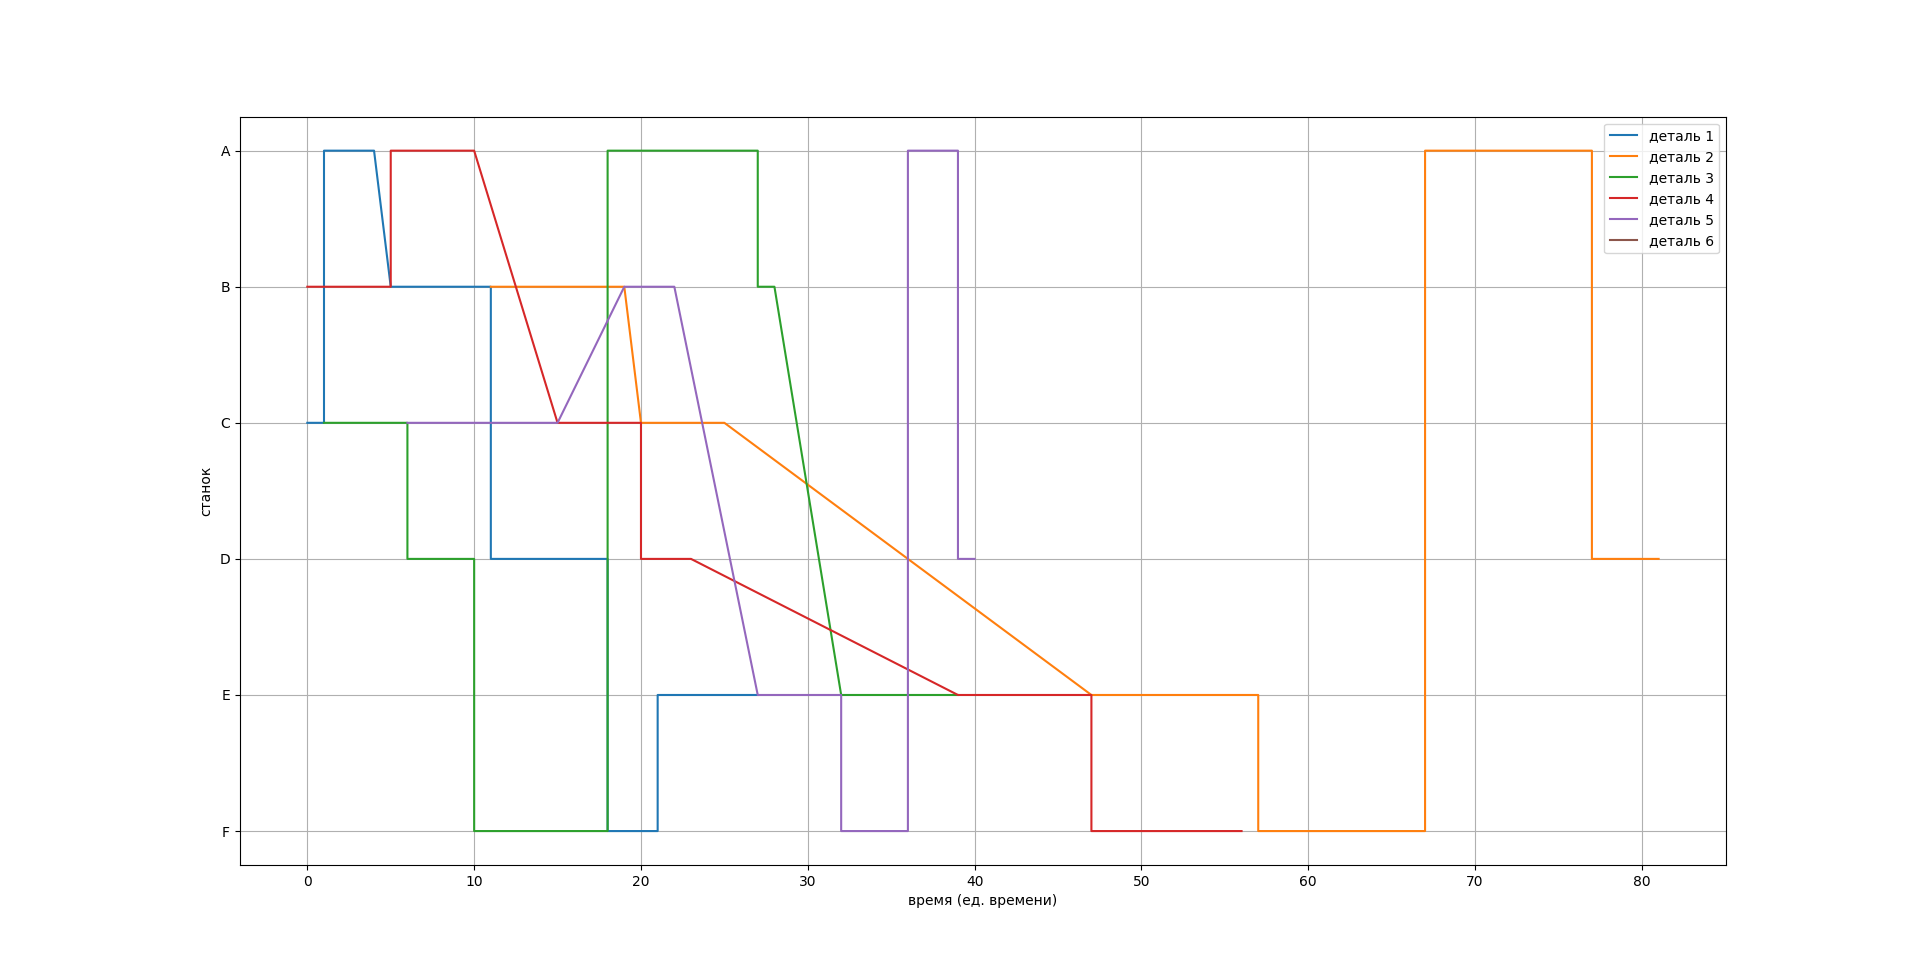
\includegraphics[width=18.25cm,height=8.5cm]{test_3.png}
      \centering
    \end{figure}
    \begin{figure}[H]
      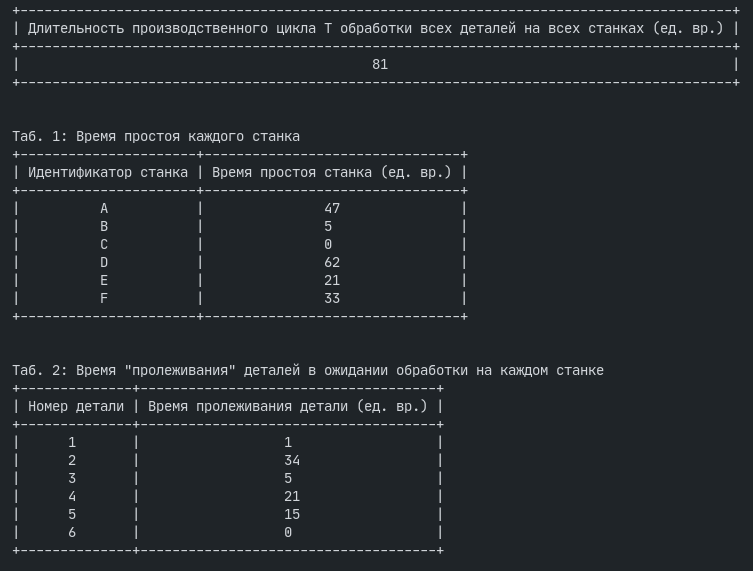
\includegraphics[width=12.25cm,height=8.5cm]{test_3_data.png}
      \centering
    \end{figure}
    \item
    \begin{figure}[H]
      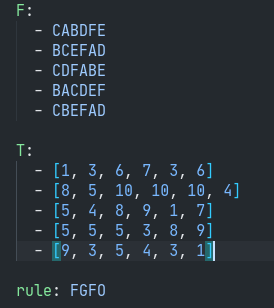
\includegraphics[width=5.25cm,height=6.5cm]{test_4_input.png}
      \centering
      \caption{\small{Модель без детали №6}}
    \end{figure}
    \begin{figure}[H]
      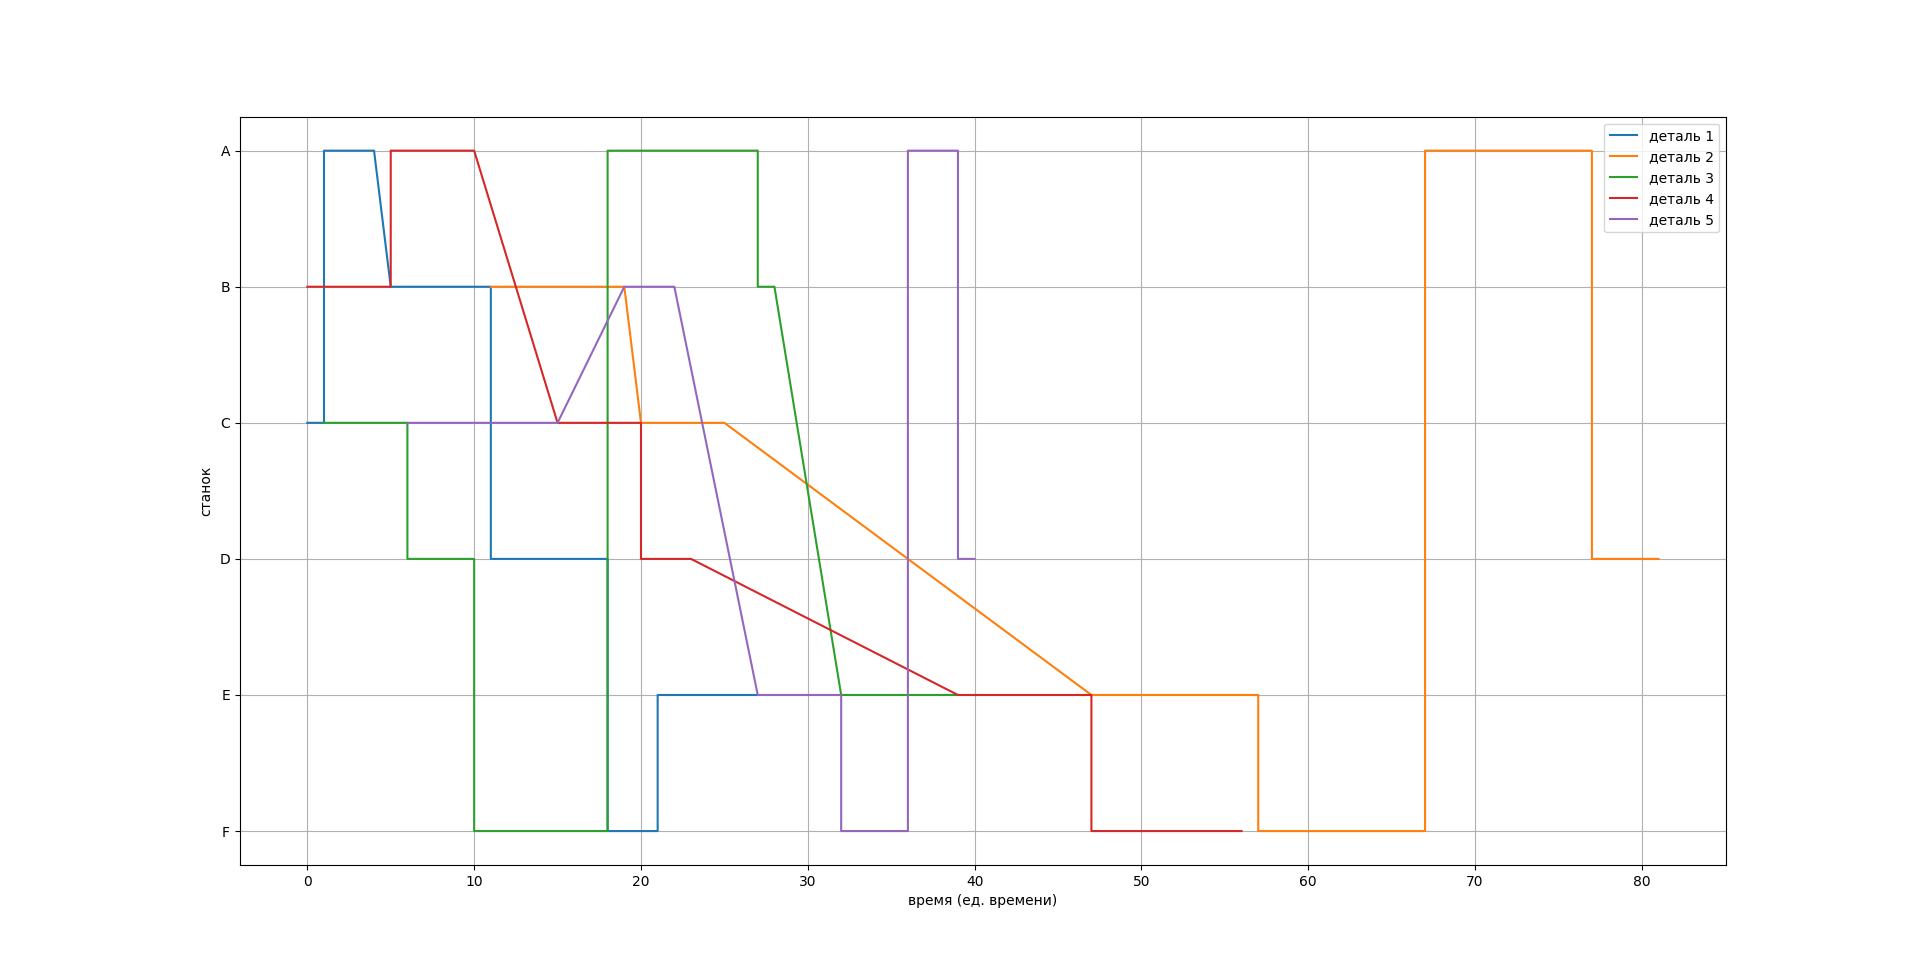
\includegraphics[width=18.25cm,height=8.5cm]{test_4.png}
      \centering
    \end{figure}
    \begin{figure}[H]
      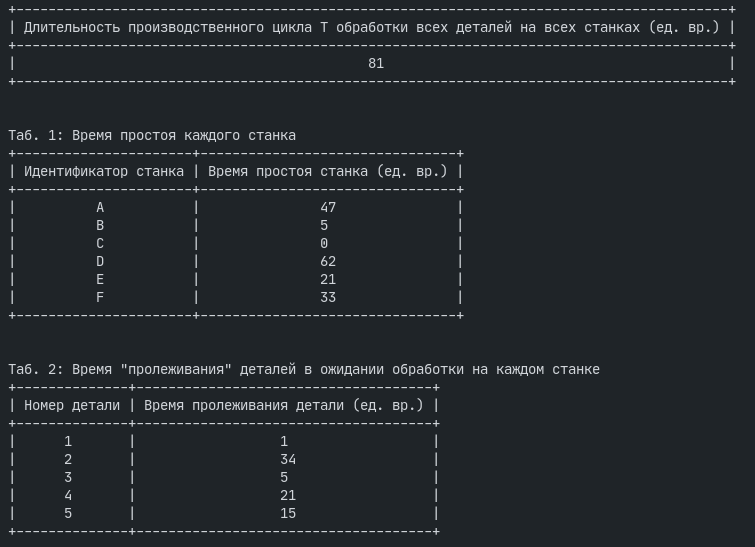
\includegraphics[width=12.25cm,height=8.5cm]{test_4_data.png}
      \centering
      \caption{\small{Как видим, параметры совпали с параметрами прошлого теста}}
    \end{figure}
    \item
    \begin{figure}[H]
      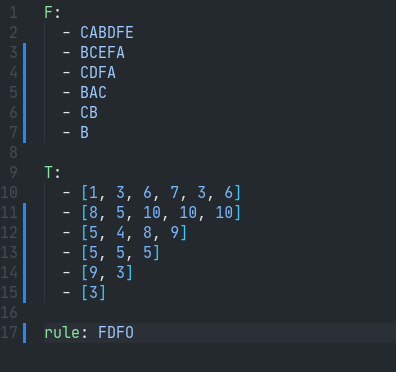
\includegraphics[width=6.25cm,height=6.5cm]{test_5_input.png}
      \centering
      \caption{\small{Модель с технологическими маршрутами разной длины}}
    \end{figure}
    \begin{figure}[H]
      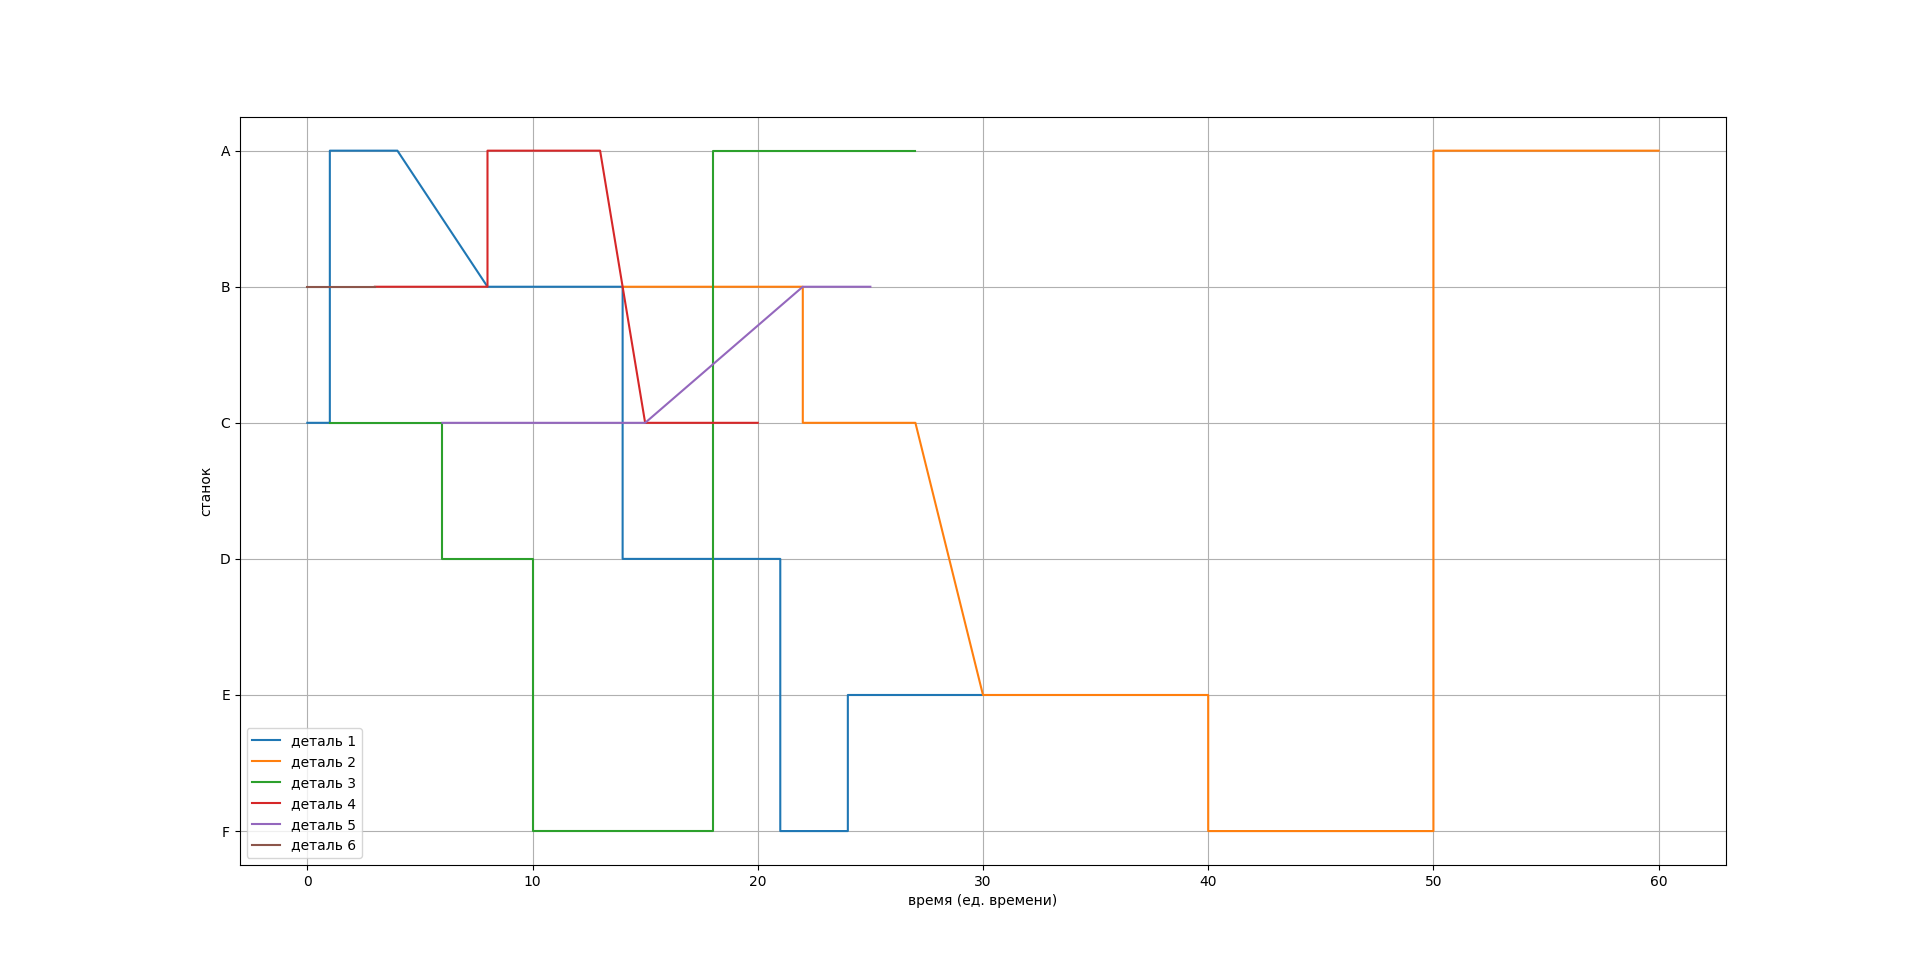
\includegraphics[width=18.25cm,height=8.5cm]{test_5.png}
      \centering
    \end{figure}
    \begin{figure}[H]
      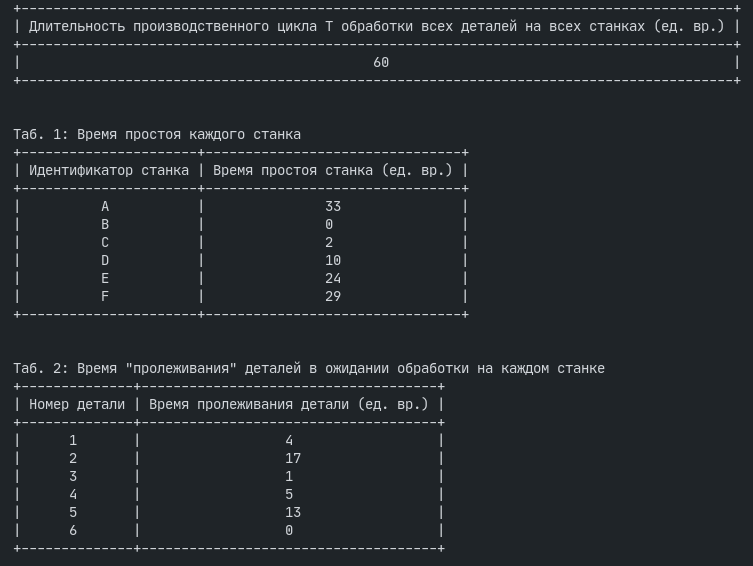
\includegraphics[width=12.25cm,height=8.5cm]{test_5_data.png}
      \centering
    \end{figure}
    \item
    \begin{figure}[H]
      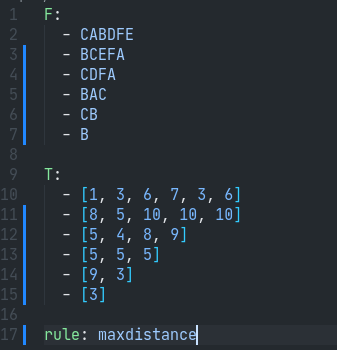
\includegraphics[width=6.25cm,height=6.5cm]{test_6_input.png}
      \centering
      \caption{\small{Модель из предыдущего теста с другим правилом предпочтения}}
    \end{figure}
    \begin{figure}[H]
      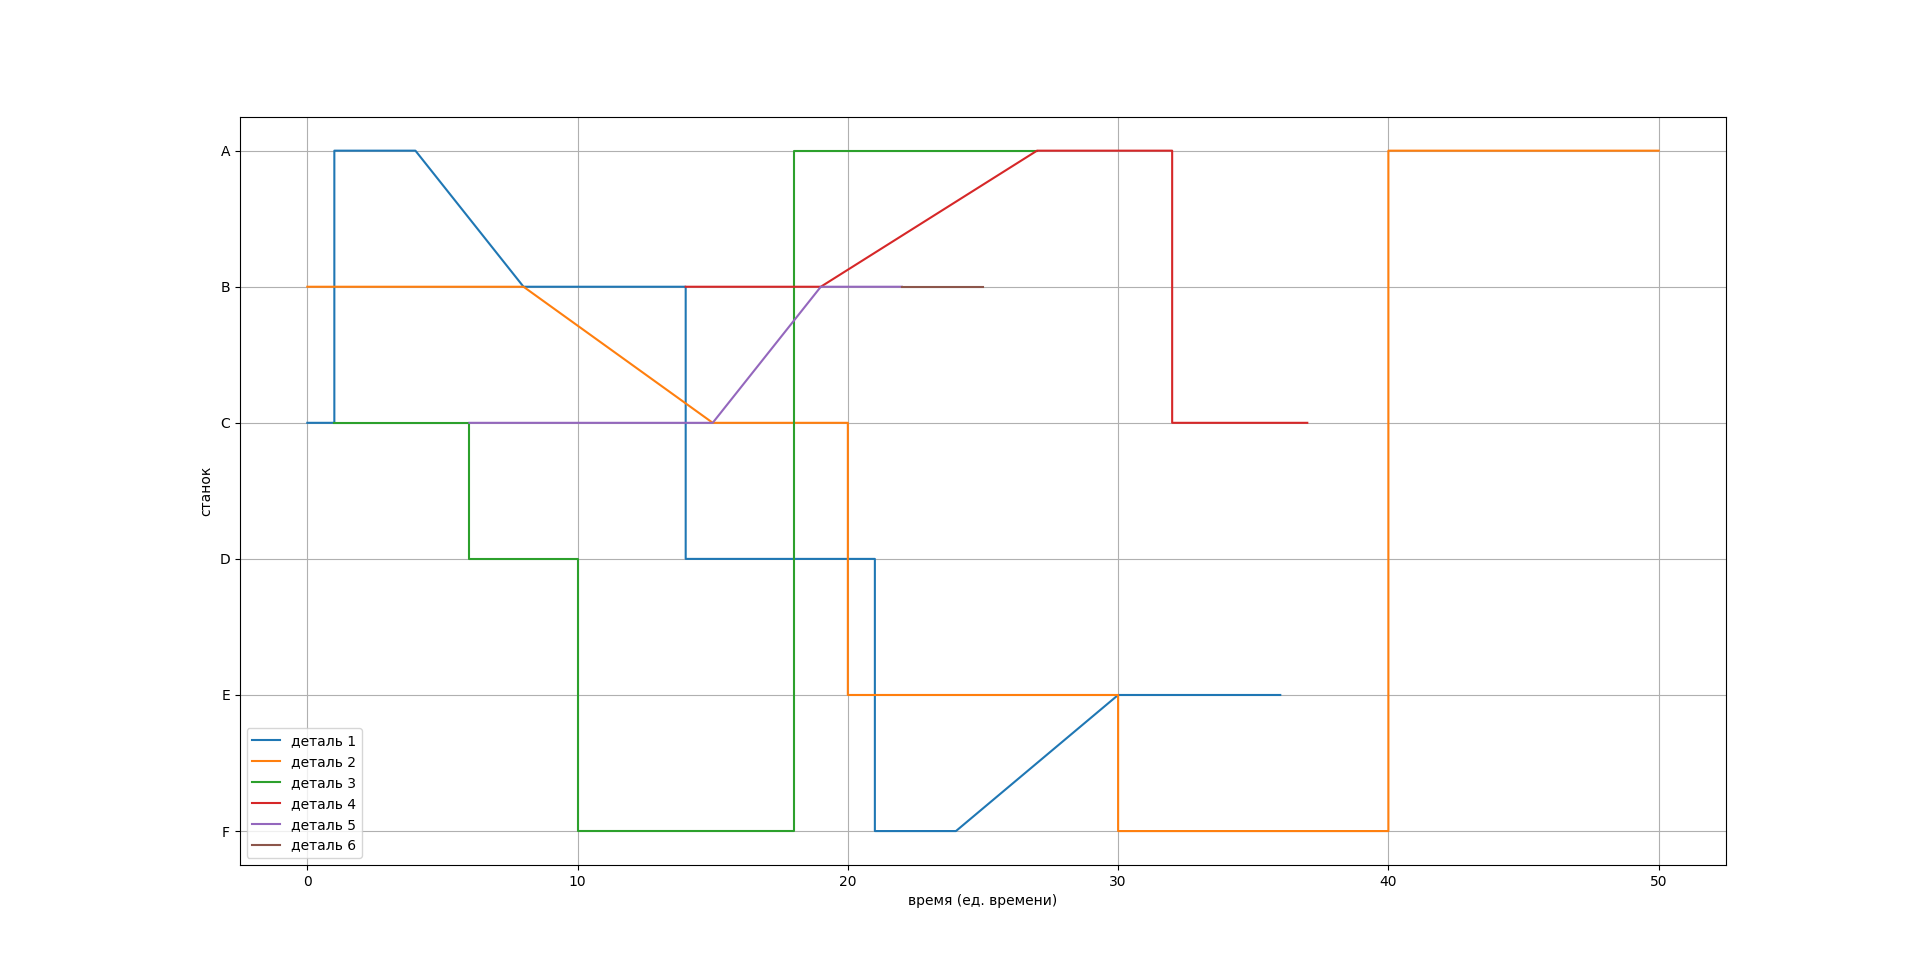
\includegraphics[width=18.25cm,height=8.5cm]{test_6.png}
      \centering
    \end{figure}
    \begin{figure}[H]
      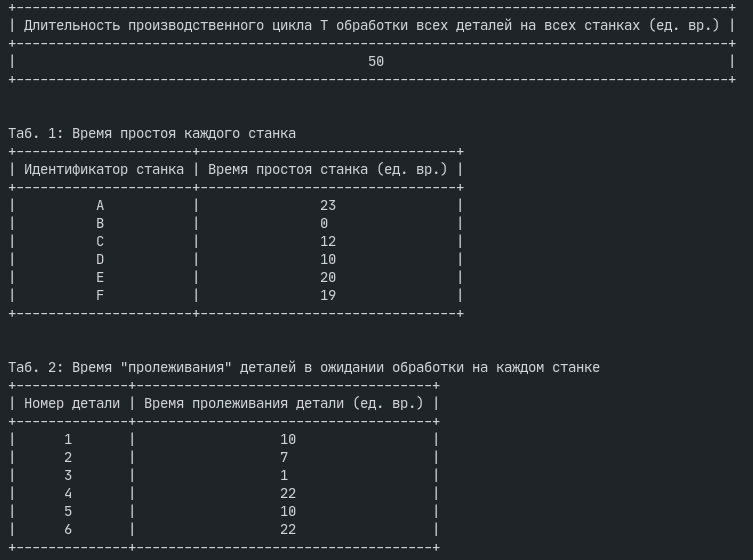
\includegraphics[width=12.25cm,height=8.5cm]{test_6_data.png}
      \centering
    \end{figure}
  \end{enumerate}
  \newpage
  \item \textbf{Сравнение показателей правил предпочтения и анализ показателей эффективности}\newline
  Возьмём для анализа модель из задания 1:\newline\linebreak
  \textbf{Запуск с правилом предпочтения "по длительности очередной операции (min.)"}
  \begin{figure}[H]
    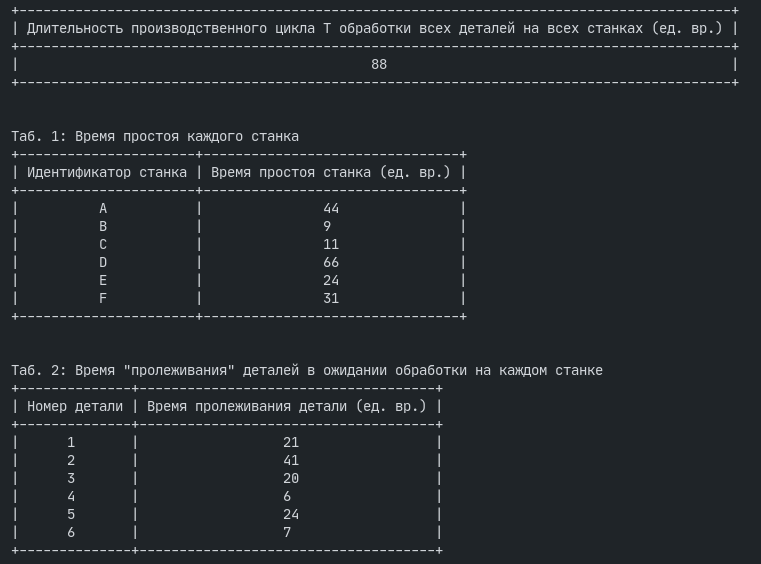
\includegraphics[width=12.25cm,height=8.5cm]{test_1_data.png}
    \centering
    \caption{}
    \label{fig:data_1}
  \end{figure}
  \begin{figure}[H]
    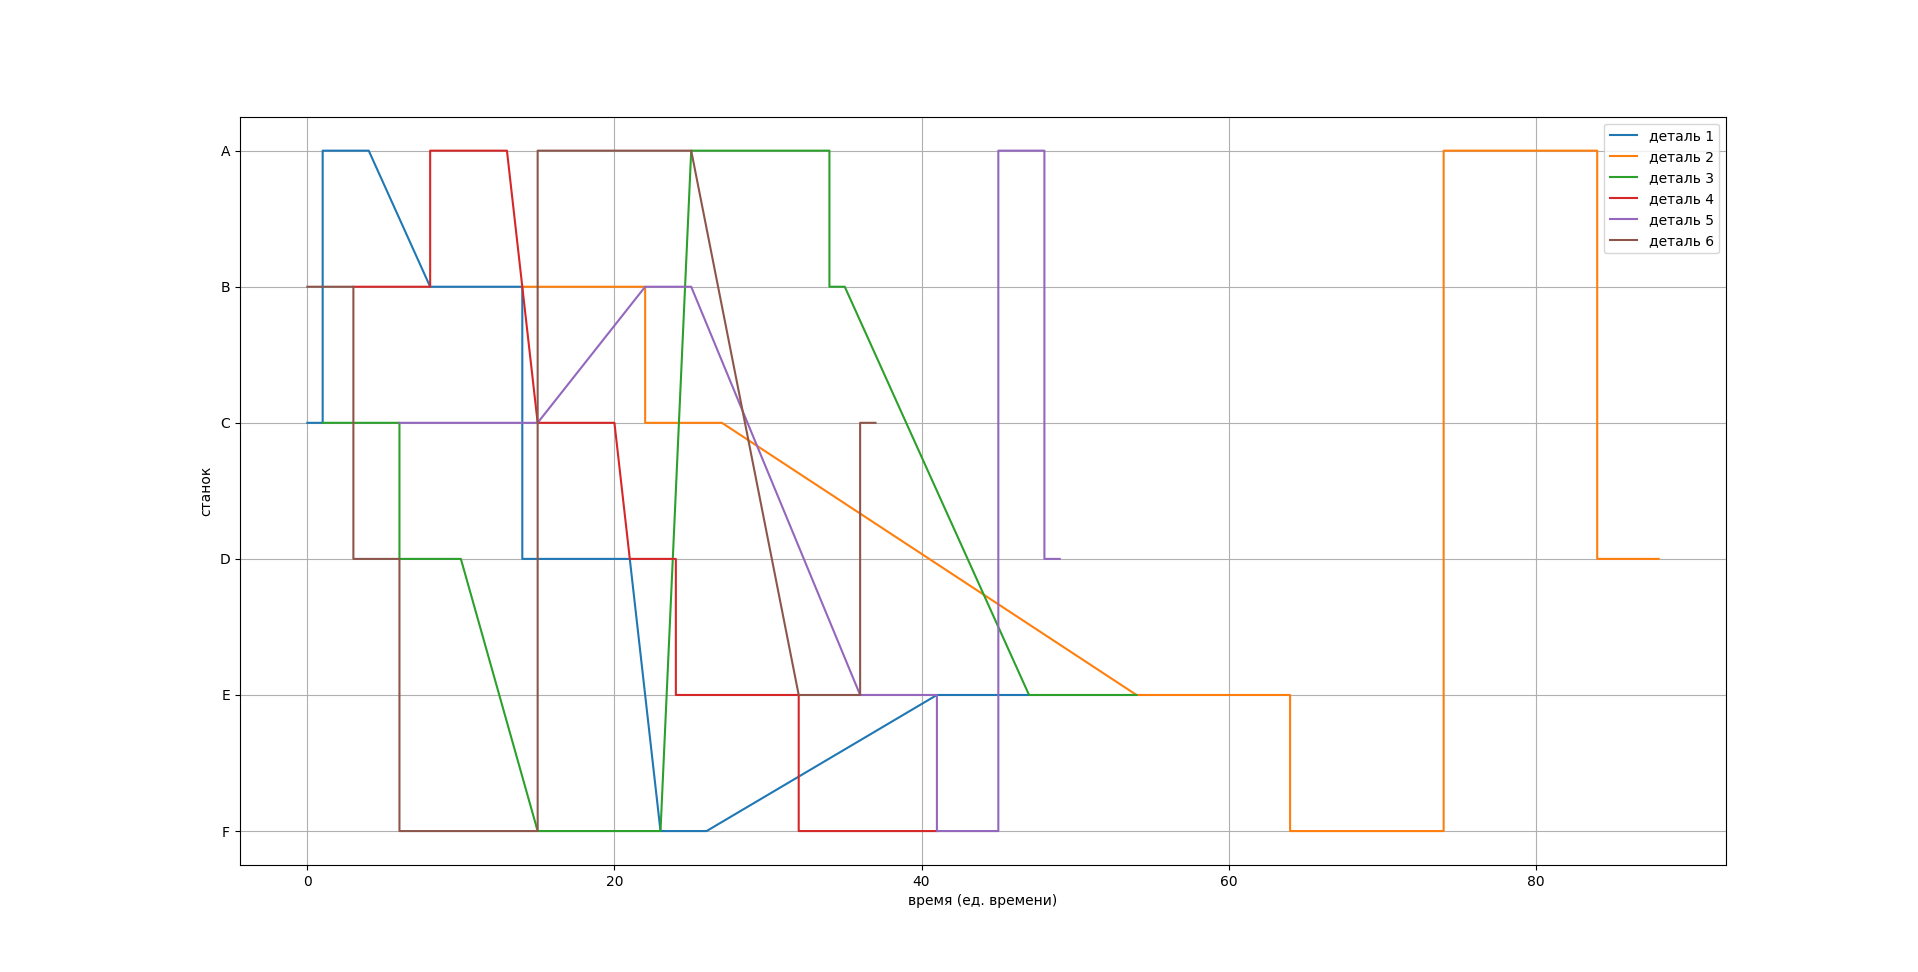
\includegraphics[width=18.25cm,height=8.5cm]{test_1.png}
    \centering
    \caption{}
    \label{fig:diagram_1}
  \end{figure}
  \textbf{Запуск с правилом предпочтения "по длительности оставшегося технологического цикла (max.)"}
  \begin{figure}[H]
    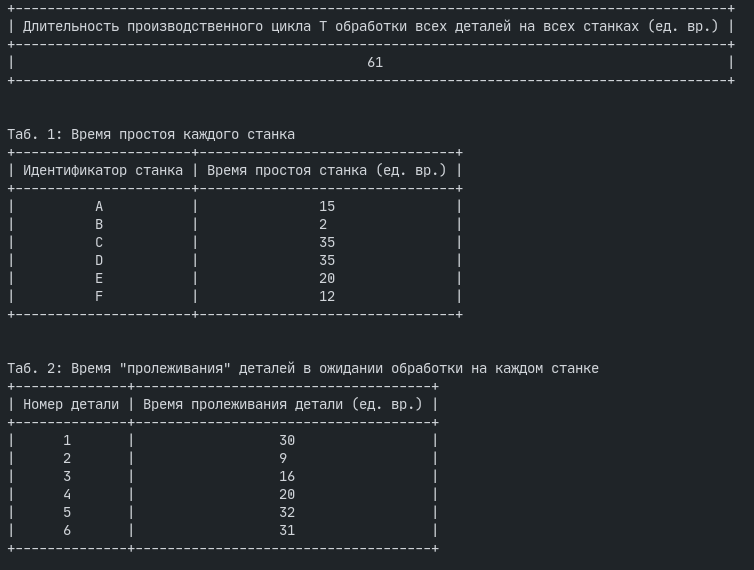
\includegraphics[width=12.25cm,height=8.5cm]{test_2_data.png}
    \centering
    \caption{}
    \label{fig:data_2}
  \end{figure}
  \begin{figure}[H]
    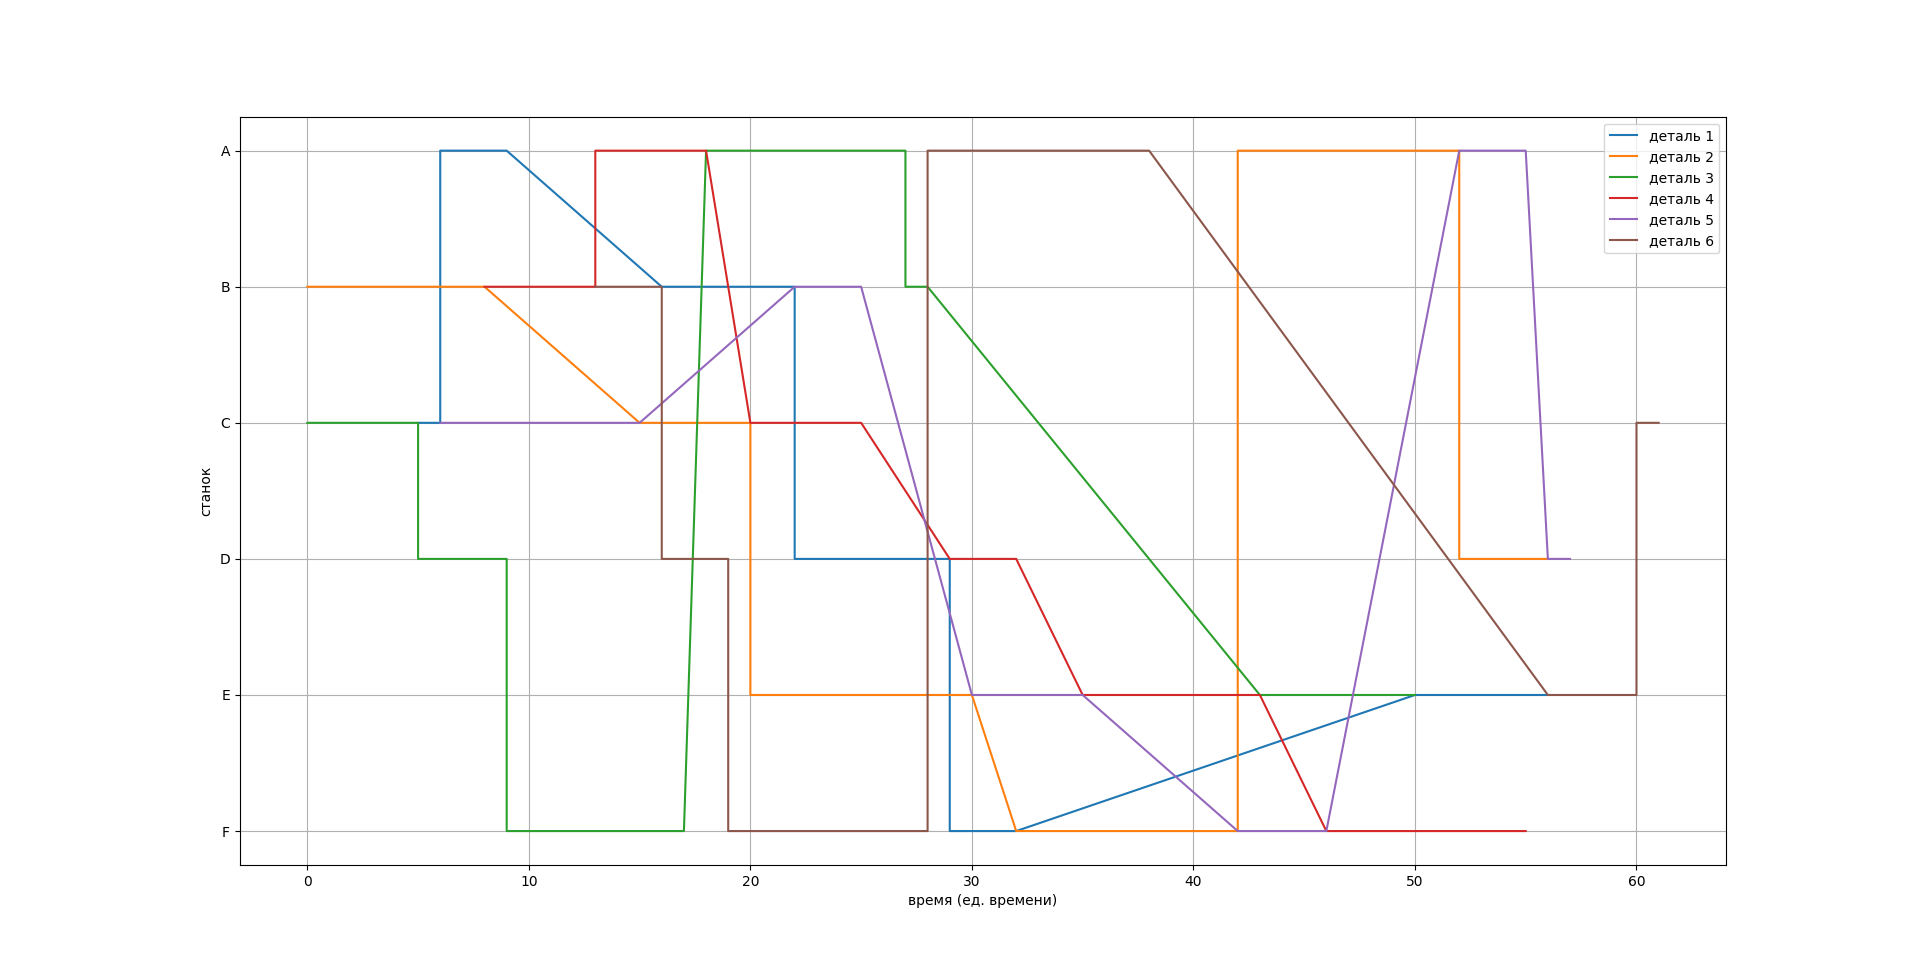
\includegraphics[width=18.25cm,height=8.5cm]{test_2.png}
    \centering
    \caption{}
    \label{fig:diagram_2}
  \end{figure}
  Обратим внимание на результаты работы программного обеспечения:
  \begin{itemize}
    \item Длительность производственного цикла Т обработки всех деталей на всех станках для правила предпочтения "по длительности очередной операции (min.)" оказалась равна \textbf{88 ед. вр.}, против \textbf{61 ед. вр.} для правила "по длительности оставшегося технологического цикла (max.)".
    \item При использовании \textit{первого} правила предпочтения, максимальное время простоя станка - \textbf{66 ед. вр.} на станке $D$, максимальное время пролеживания детали - \textbf{41 ед. вр.} для детали №2.\newline\textbf{Суммарное время простоя станков: 185 ед.вр.}, \textbf{Суммарное время пролеживания деталей: 119 ед.вр.}
    \item При использовании \textit{второго} правила предпочтения, максимальное время простоя станка - \textbf{35 ед. вр.} на станках $C$, $D$, максимальное время пролеживания детали - \textbf{32 ед. вр.} для детали №5.\newline\textbf{Суммарное время простоя станков: 119. ед. вр}, \textbf{Суммарное время пролеживания деталей: 138 ед.вр.}
  \end{itemize}
  На рис. \ref{fig:diagram_1} видно, что часть производственного цикла для детали №2 обрабатывается в последнюю очередь. Нормы времени для этого промежутка (ед. вр.): 10, 10, 10, 4. Так как по правилу предпочтения выбирается очередная операция с \textit{миниальной нормой выполнения}, очевидно, что детали с нормой на выполнение в 10 единиц остаются в конце производственной очереди. Этим объясняется б\emph{о}льшая длительность производственного цикла.\newline\linebreak
  Как видно на рис. \ref{fig:data_1}, \ref{fig:diagram_1}, б\emph{о}льший вес в суммарном времени простоя станков имеют станки $A, D$ (44. ед. вр. и 66. ед. вр. соотв.). На рис. \ref{fig:diagram_1} видно, что станок $A$ простаивает значительное время между загрузками детали №5 и детали №2. Станок $D$ простаивает более половины производственного процесса с выгрузки детали №4 до загрузки детали №2. Эти простои - следствие обработки "времязатратной" части детали №2 в последнюю очередь.
  \newline\linebreak
  Самая "неактивная" деталь №2 пролеживает всё также потому, что не является приоритетной в очереди по длительности следующей операции. Задержка другого характера - позднее начало обработки (деталь №5, 24. ед. вр. пролеживания) - тоже результат формирования очереди, так как деталь с нормой времени 9 попадает на станок $C$ не сразу, после деталей №1 и №3 с нормами времени 1 и 5 для станка $C$ соответственно.
  \newline\linebreak
  Из анализа организации производственной очереди по первому правилу предпочтения можно сделать вывод, что системы с достаточно большими дельтами норм времени не обязательно будут организованы \textit{оптимально}, так как времязатратные операции будут выбираться в последнюю очередь, что ведёт к двум проблемам: поздней подаче элемента на производственный конвейер и позднему завершению обработки на конвейере.
  \newline\linebreak\linebreak\linebreak
  Правило предпочтения "по длительности части технологического цикла, операции по которому осталось выполнить (max.)"$~$устраняет проблему из первого случая, так как считает приоритетными наиболее "времязатратные" $~$ маршруты, тем самым делая невозможной ситуацию, когда самые "длинные" $~$ операции обрабатываются в производственном цикле в последнюю очередь.
  \newline\linebreak
  Недостатком второго правила можно считать тот факт, что выбор \textit{явным} образом не основывается на очередной операции, и поэтому детали могут поступать на первичную обработку позднее, чем они поступали в первом случае. Например, на станок $B$ поступает деталь №2 с нормой времени 8. ед. вр., вынуждая детали №4, №6 пролеживать, хотя с первым правилом они бы уже поступили на другой станок. Кроме прочего, задержки в начале влияют и на дальнейшее состояние системы, детали №4, №6 пролеживают, пока обрабатывается деталь №2 на станке $B$, только после обработки этих деталей на $B$ может поступить деталь №1, часть времени обработки деталей №4, №6 образует время пролеживания детали №1, связанное с переходом из обработки на станке $A$ на обработку на станке $B$.
  \newline\linebreak
  Еще одним недостатком является то, что часть технологического цикла обработки детали может выполняться в последнюю очередь, так как с определенного времени оставшиеся операции по маршруту будут малы по времени в сравнении с другими технологическими маршрутами. Так, деталь №6 при наличии "времязатратных" операций обрабатывается своевременно, но когда в маршруте остаются операции стоимостью 4 и 1 ед. вр., приоритет маршрута понижается, и деталь обрабатывается до конца в последнюю очередь; что влечёт за собой появление значительного интервала пролеживания, простоя станка.
  \newline\linebreak
  Можно сделать вывод, что второе правило предпочтения следует использовать в системах с \textit{равномерным} распределением норм времени по маршруту (все временные отрезки на маршруте примерно одинаковые).
\end{enumerate}
\end{flushleft}

\end{document}
